% Learned correction layer: the MLP that predicts an ILC table from path geometry.
% Same black & white paper style as model_schematic.tex / method_loop.tex.
\documentclass[border=6pt]{standalone}
\usepackage{tikz}\usepackage{amsmath}
\usetikzlibrary{arrows.meta,positioning,calc,fit}
\begin{document}
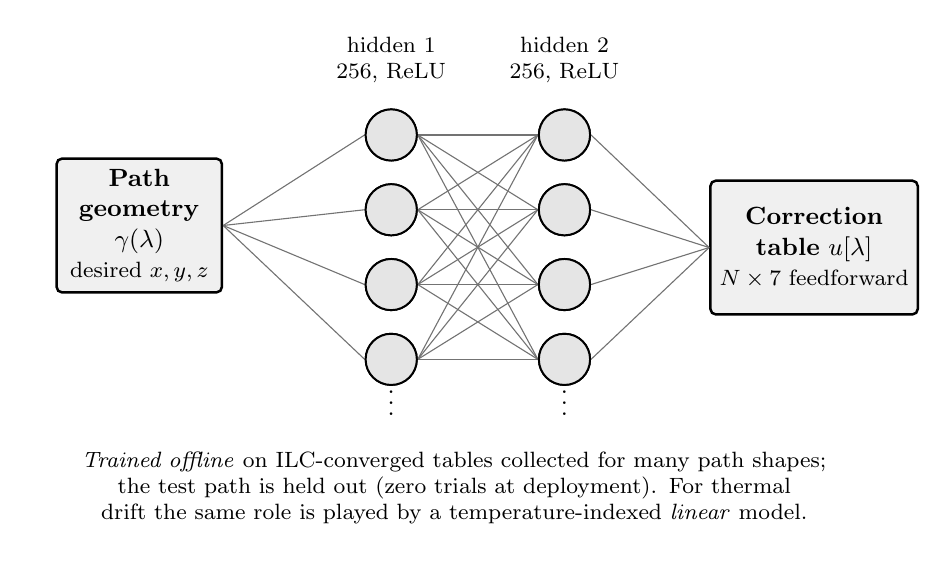
\begin{tikzpicture}[font=\small,>={Latex[length=2.0mm]},
  io/.style={draw=black,line width=0.9pt,rounded corners=2pt,align=center,
             minimum height=1.7cm,minimum width=2.1cm,fill=black!6},
  neuron/.style={draw=black,line width=0.7pt,circle,minimum size=6.5mm,fill=black!10},
  lab/.style={font=\footnotesize,align=center},
  conn/.style={draw=black!55,line width=0.4pt}]

% ---- input block ----
\node[io] (in) {\textbf{Path}\\\textbf{geometry}\\$\gamma(\lambda)$\\{\footnotesize desired $x,y,z$}};

% ---- hidden layer 1 (4 representative units of 256) ----
\foreach \i in {1,...,4}
  \node[neuron] (a\i) at (3.2, 2.1-0.95*\i) {};
\node[lab,above=2mm of a1] {hidden 1\\$256$, ReLU};

% ---- hidden layer 2 ----
\foreach \i in {1,...,4}
  \node[neuron] (b\i) at (5.4, 2.1-0.95*\i) {};
\node[lab,above=2mm of b1] {hidden 2\\$256$, ReLU};

% ---- output block ----
\node[io,right=1.5cm of b2.east,yshift=-0.48cm] (out)
  {\textbf{Correction}\\\textbf{table} $u[\lambda]$\\{\footnotesize $N\times7$ feedforward}};

% ---- connections (fully connected) ----
\foreach \j in {1,...,4} \draw[conn] (in.east) -- (a\j.west);
\foreach \i in {1,...,4}\foreach \j in {1,...,4} \draw[conn] (a\i.east) -- (b\j.west);
\foreach \i in {1,...,4} \draw[conn] (b\i.east) -- (out.west);

% redraw nodes on top of the wires
\foreach \i in {1,...,4}{\node[neuron] at (a\i){};\node[neuron] at (b\i){};}

% ---- vdots to signal "256, not 4" ----
\node at (3.2,-2.15) {$\vdots$};
\node at (5.4,-2.15) {$\vdots$};

% ---- training / scope note ----
\node[lab,anchor=north,text width=10.6cm] at (4.0,-2.75)
 {\emph{Trained offline} on ILC-converged tables collected for many path shapes;
  the test path is held out (zero trials at deployment). For thermal drift the
  same role is played by a temperature-indexed \emph{linear} model.};
\end{tikzpicture}
\end{document}
